\documentclass[10pt,twocolumn]{article}

% use the oxycomps style file
\usepackage{oxycomps}
\usepackage{enumitem}
\usepackage{graphicx}


% usage: \fixme[comments describing issue]{text to be fixed}
% define \fixme as not doing anything special
\newcommand{\fixme}[2][]{#2}
% overwrite it so it shows up as red
\renewcommand{\fixme}[2][]{\textcolor{red}{#2}}
% overwrite it again so related text shows as footnotes
%\renewcommand{\fixme}[2][]{\textcolor{red}{#2\footnote{#1}}}

% read references.bib for the bibtex data
\bibliography{references}

% include metadata in the generated pdf file
\pdfinfo{
    /Title (The Occidental Computer Science Comprehensive Project: Goals, Timeline, Format, and Advice)
    /Author (Justin Li)
}

% set the title and author information
\title{Junior Comps Proposal: \\ Web Application For Dining Review }
\author{Rui Chai}
\affiliation{Occidental College}
\email{rchai@oxy.edu}

\begin{document}

\maketitle

\section{Introduction}
In this project, I propose to develop a web application that supports functions similar to Yelp but is simplified for ease of use and customized for the needs of Occidental College students, faculties, and local community members. The primary focus of this application will be to provide a platform where users can easily access, write, and share reviews of local dining facilities, contributing to better consumer experiences and improving dining services.

The idea for this project stems from the observation that while comprehensive platforms like Yelp offer a wide range of features, they can sometimes be overwhelming for users who are only interested in basic functionalities such as reading and posting reviews. Additionally, these platforms are open to the general public, which have less relevance to the content for the Occidental communities. There is a need for a more focused application that prioritizes ease of use and accessibility, particularly for those who prefer simpler applications, or prefer sharing their opinions within a smaller and closer community.

The application will thus be designed with a clean, user-friendly interface concentrating on the core aspects of a review platform. It will contain core features such as create accounts, search for out-of-campus restaurants, and post reviews. Users will also be able to rate dining facilities and see an aggregate of user ratings, which will help them make informed choices about dining.

The goal of this project is not only to develop a functional application, but also to engage with and contribute to the Occidental community by enhancing the accountability of dining facilities. By providing a platform tailored to the needs of a specific user group, the project will offer a more personalized and relevant experience for its users.

This proposal will outline the problem context that motivates the project, provide a technical background on the methodologies and technologies to be used, review prior work in this area, describe the methods and approaches for development and evaluation, and finally, present a detailed timeline for the completion of the project. Through this development process, I aim to gain practical experience in web application development while offering a valuable tool to the community.

\section{Problem Context}
Review websites and apps like Yelp have become extremely popular and influential in recent years. Consumers regularly use these platforms to read reviews and make decisions about which local businesses to visit or services to use. However, there are several major issues with existing review platforms that undermine their usefulness and accessibility for the Occidental College community.

One of the biggest problems is that large review platforms like Yelp do not cater specifically to the needs of students at universities. These platforms typically aim to cover a broad spectrum of businesses and services, which can result in reviews that lack depth or specific details relevant to student life. Specifically, Yelp or Google Maps does not provide sufficient information and consumer reviews for the dining facilities at Occidental. For instance, new students may be looking for information on the best cuisines at the Oxy Marketplace, or late-night eateries at the Tiger Cooler. These details are often missing in broader reviews, and hard to obtain from non-student users. This disconnect highlights the necessity for a more customized solution that addresses the unique preferences and concerns of the Occidental community.

The prevalence of fake or misleading reviews is another big problem. Businesses sometimes hire companies or individuals to post large numbers of positive reviews to artificially inflate their ratings. Conversely, rivals may flood a business's page with unjustified negative reviews. While the platforms claim to use filtering algorithms, clearly many fake reviews still exist. A research "identified a significant correlation between the visual browsing behavior of consumers and their purchase intention and found that consumers were not able to identify false comments." (Chen 2022) This makes it extremely difficult for consumers to get an accurate sense of a business's quality.

Another issue is the lack of accountability and transparency among the campus dining facility operations. Students often encounter issues with food quality, service, and availability, yet there are insufficient channels for them to provide feedback or voice concerns. This absence of a structured feedback mechanism leads to frustration and a feeling of disconnect between students and dining services, ultimately affecting student satisfaction and the overall dining experience on campus.

To address these problems, I propose developing a community-driven review platform specifically focused on Occidental College and local businesses in our area. By putting more control in the hands of individual users rather than a centralized corporate entity, we can increase transparency and build a more trustworthy source of dining information and feedback mechanism.

\section{Technical Background}
This section provides an overview of the technical foundations necessary for the development of this web application. A typical web application consists of three main components: the front end (client side), the back end (server side), and the database. 



The front end handles what the users can see and interact with. For example, creating reusable UI components for common elements like business listings, review cards, navigation menus. For this project, the front end will be developed using HTML, CSS, and JavaScript, the basic technologies for web content. We use React, a JavaScript library for building user interfaces, to create a responsive and dynamic experience. The frameworks are chosen based on their ability to handle specific project requirements such as rapid development, scalability, security, and full-stack development capabilities. (BrowserStack)

The back end handles the core operational logic of the application, processing user requests, and performing actions such as database operations. We will use the Node.js JavaScript runtime to build the back end. It allows for the development of scalable network applications. We may also integrate with third-party APIs to fetch supplemental data.

The database will store all data related to users and business reviews. In the early developing and testing stage, we will use Google Firebase as a temporary database platform due to its ease of use and our previous experiences. MongoDB, a NoSQL database, is chosen for later use on the actual application because of its flexibility and ease of integration with JavaScript. It will store data in JSON documents, which supports the potential data structure used in the application.

To facilitate the functionality of searching and sorting business reviews, basic algorithms like quicksort for sorting and binary search for querying specific data efficiently will be implemented. These algorithms are chosen for their efficiency in handling large datasets, which is crucial as the database grows with more user reviews, and their ease to implement that fits our current CS knowledge level.

To ensure data integrity and secure user interactions, the application will incorporate standard security and authentication practices. Hashing algorithms, such as SHA-256, will be used to safely store user passwords. HTTPS will be implemented to secure data transmission between the client and the server. Access to the database and user data will be strictly constrained and will not be shared or sold to any third party. These measures prevent unauthorized access and ensure that user data is protected.

For alternative front end libraries, we may consider choosing between React and jQuery. We may include Flutter to take advantage of its ideas of widgets when building the web page. On the back end, although Node.js provides a robust environment for server-side logic, Spring Boot is still an alternative because learning it prepares us with more enterprise-level skills.

For databases, Google Firebase offers several cloud services, including authentication, real-time database, cloud storage, cloud functions, and analytics. However, we wish to learn more database skills and don’t want to pay for Google, so we will replace Firebase with other SQL such as MongoDB soon after we understand how it works. 

\section{Prior Work}
This section examines existing solutions and research related to web applications for business reviews and recommendations. This section highlights the strengths and weaknesses of current platforms and identifies gaps that the proposed project aims to fill. This review helps us to understand what kind of application is already developed and to ensure our proposed solution brings novel contributions to the existing landscape.

\subsection{Review Platforms}
\begin{enumerate}
    \item \textbf{Yelp} As one of the most recognized platforms for business reviews, Yelp offers extensive features including user reviews, business information, and social networking elements. However, its complex interface, excessive contents and commercialization (e.g., paid reviews and advertisements) can detract from user experience and trust.
    
    \item \textbf{Google Reviews} Integrated within Google Maps, this platform provides convenience and accessibility for Google’s massive user base. While highly accessible, it lacks certain features that could enhance user engagement, such as detailed user profiles and social interactions among users.
    
    \item \textbf{TripAdvisor} As a Yelp alternative, it focused primarily on travel-related services, TripAdvisor combines reviews with booking capabilities. Its niche focus is both a strength and a limitation, as it does not cater to all types of businesses.
    \end{enumerate}
    All these platforms, especially Yelp and Google Reviews, are prominent in the landscape of online business reviews. Yelp's community-focused model supports detailed, personal reviews which are especially influential in the hospitality and service industries. On the other hand, Google Reviews' integration with search results makes it a powerful tool for businesses seeking broad visibility and direct impact on search rankings. (B12.io)

    \section{Methods}
    This section includes the design and implementation strategies, data handling processes, and the tools and technologies to be used. We also explore potential alternative methods besides the chosen approach.
    
    \subsection{Development Tools and Technologies}  
\begin{enumerate}    
        \item \textbf{IDE} VSCode
        \item \textbf{Version Control} Git will be employed for version control, with GitHub used for repository hosting and collaboration.
        \item \textbf{Testing Frameworks} For frontend, Jest and React Testing Library for unit and integration testing of React components. For backend, Mocha and Chai for testing server-side logic and API endpoints.
\end{enumerate}

\subsection{Development Methodologies}
We can choose the Agile frameworks for their flexibility, customer-centric approach, and ability to adapt to changes rapidly. These methodologies support iterative development cycles, emphasizing continuous feedback and collaboration among cross-functional teams, making them suitable for projects where requirements may evolve over time. (FreeCodeCamp)

    \subsection{Web-page Design}
    \begin{enumerate}
        \item \textbf{UI Design} The UI will be divided into reusable components such as the header, footer, navigation bar, business listing, review form, and user profile. Each component will be designed to be visually consistent and functionally straightforward.
Initial wireframes will be created to outline the basic layout of the application. These wireframes will focus on simplicity and usability, ensuring that users can easily navigate the app. We will gather feedback from surveys and perfect the prototype through rapid iteration. 
        \item \textbf{UX Design} Users will be able to register and log in using a simple form. Passwords will be hashed before storage to ensure security. Users can search for businesses by name or category. Filters will allow users to sort businesses by rating, location, or review date. Users can submit reviews via a form that includes fields for rating, comments, and optional photos. Validation will ensure that all required fields are completed before submission.      
    \end{enumerate}

    \begin{figure}
    \centering
    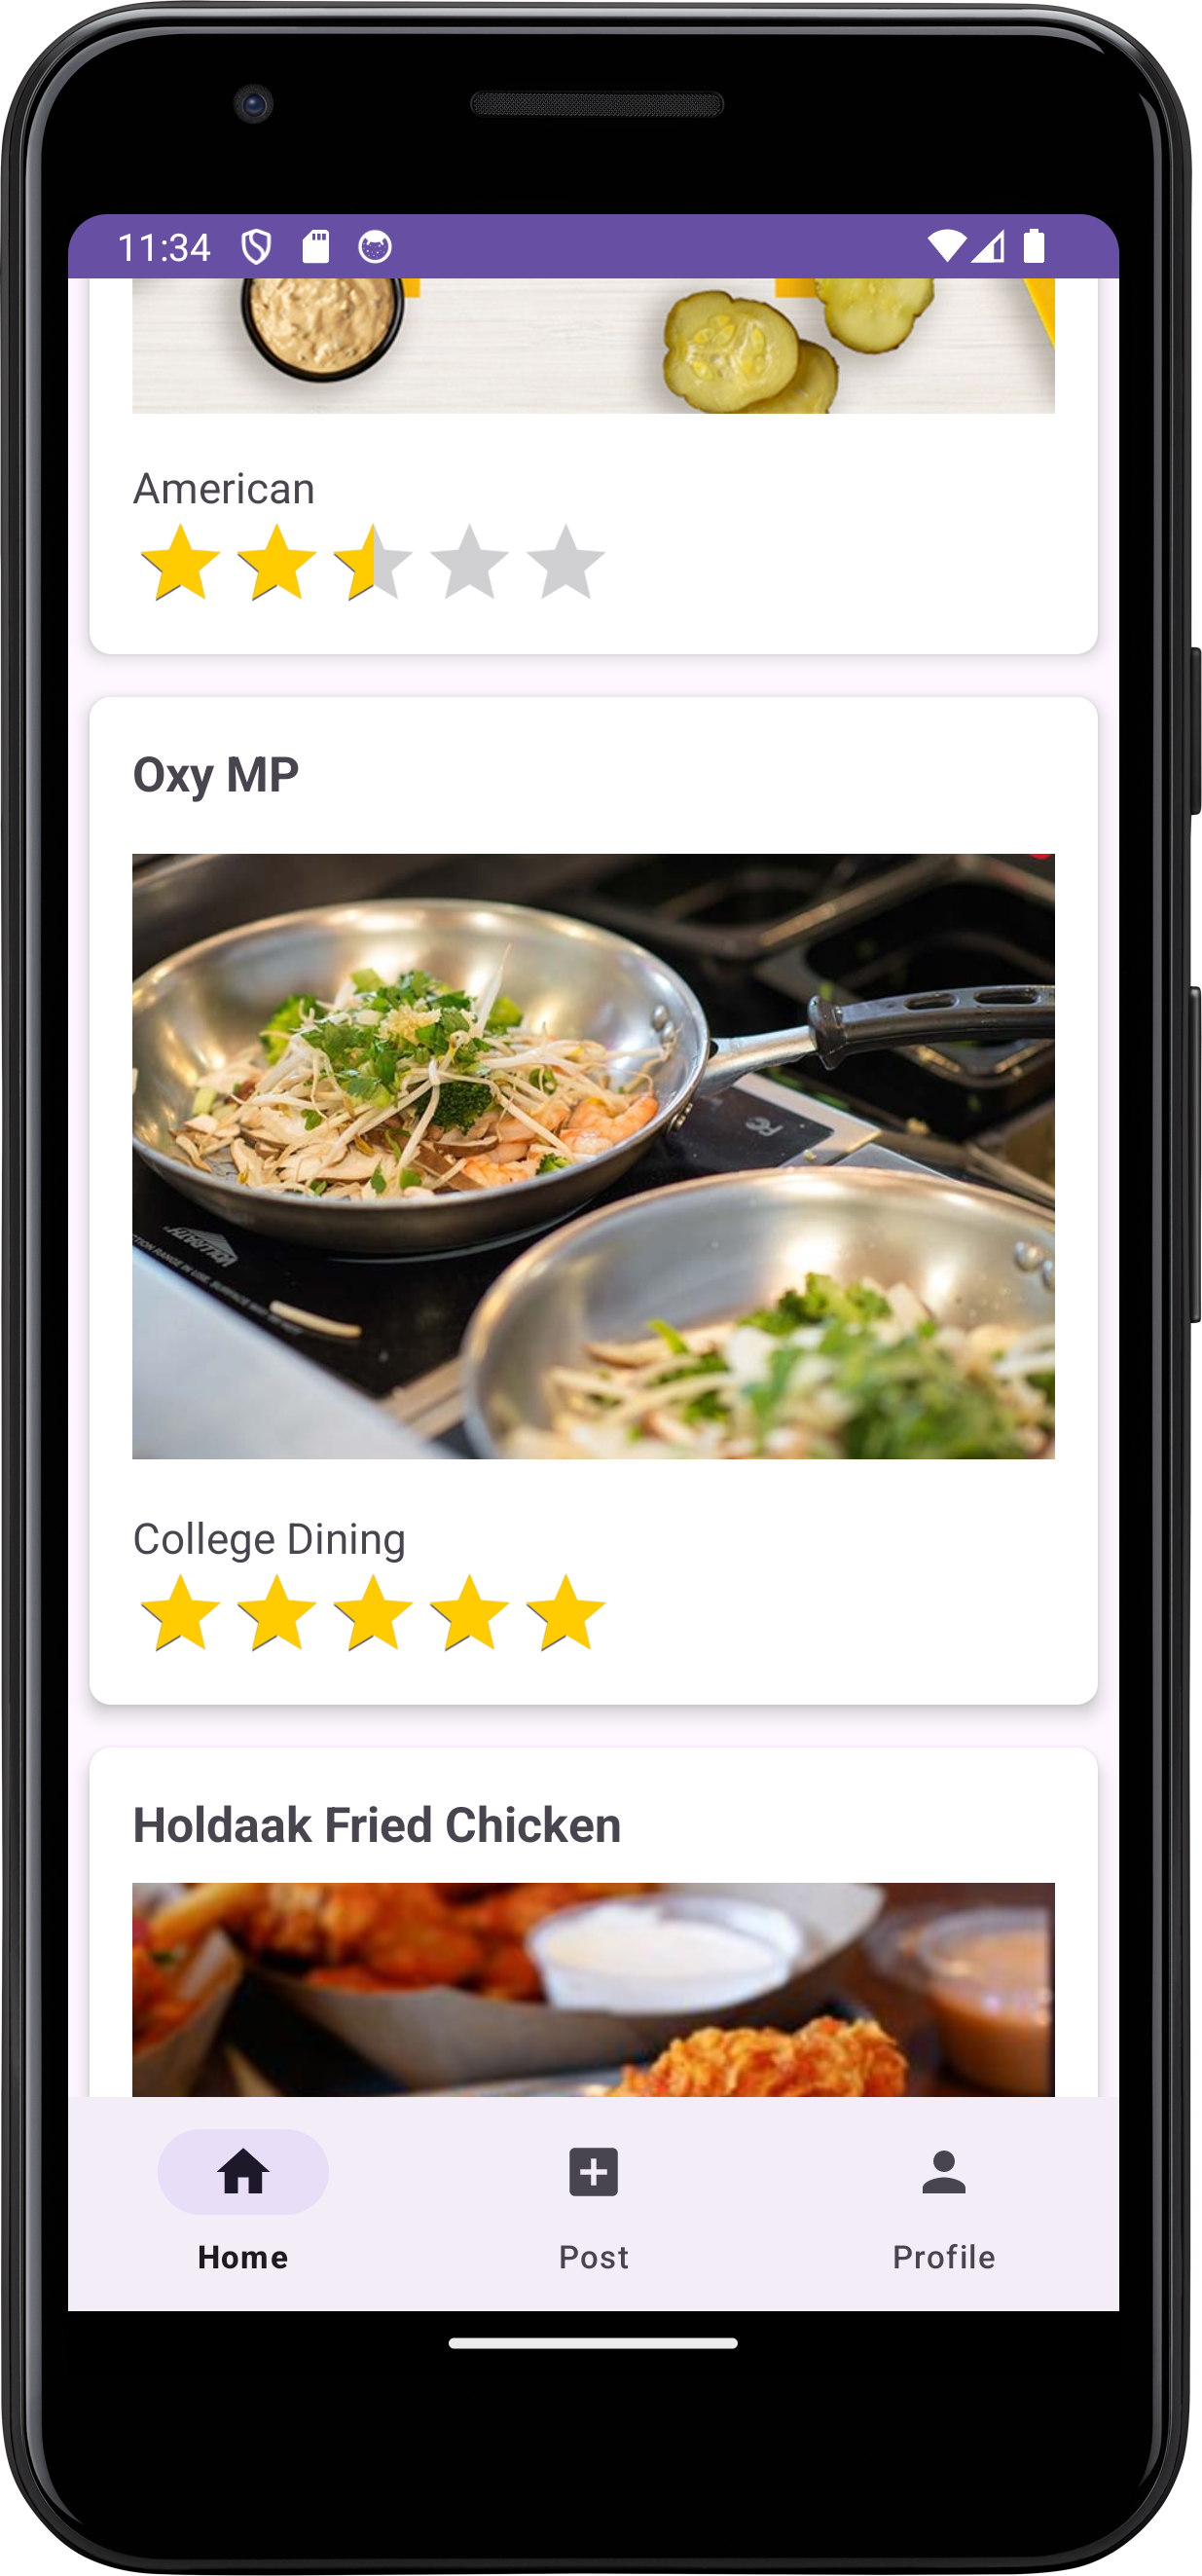
\includegraphics[width=\linewidth]{SampleAndroidPage.png}
    \caption{Sample Android Page}
    \label{fig:my_label}
   \end{figure}

       \begin{figure}
    \centering
    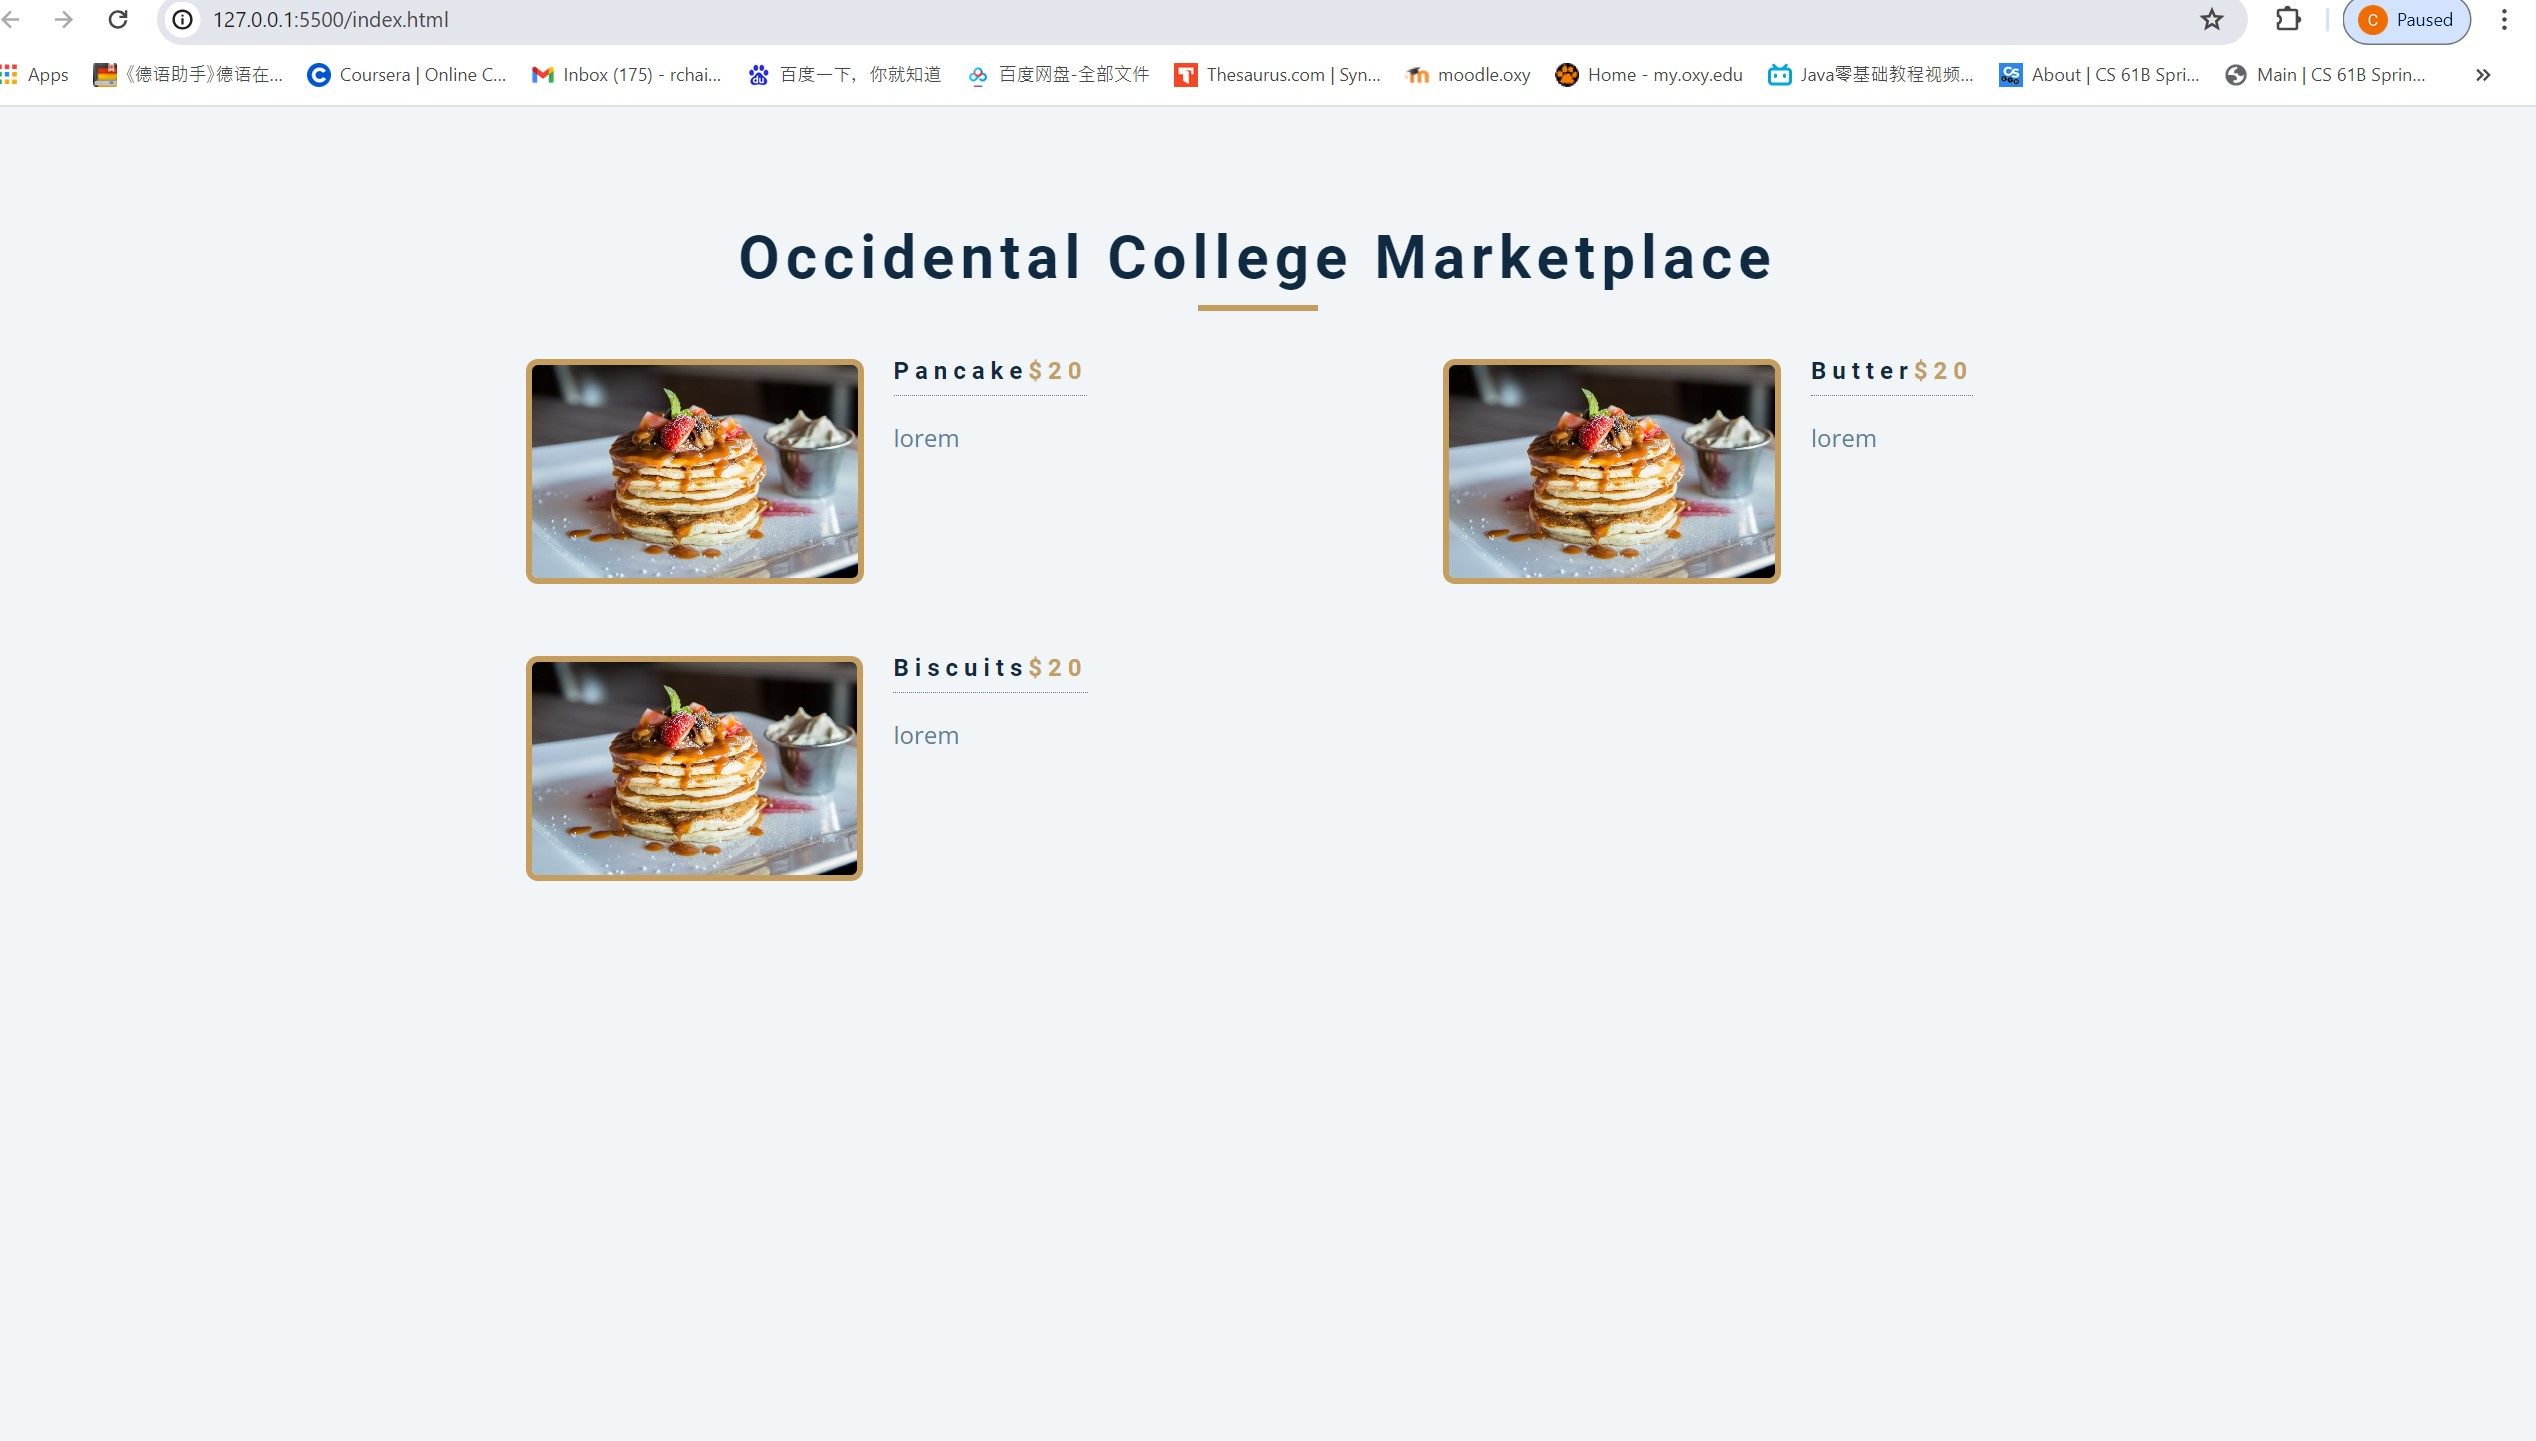
\includegraphics[width=\linewidth]{SampleWebpage.jpg}
    \caption{Sample Web Page}
    \label{fig:my_label}
   \end{figure}

    \subsection{Functionalities}
    \subsubsection{Front End}
    \begin{enumerate}
        \item Homepage showing popular/trending local businesses 
        \item Search interface for querying businesses by name/category/location
        \item Business profile pages displaying details, photos, map, reviews
        \item User profile pages showing their reviews, lists, profile settings
        \item Authentication flows for signing up, logging in 
        \item Other advanced features

    \end{enumerate}
    \subsubsection{Back End}
    \begin{enumerate}
        \item User account management
        \item CRUD operations for business listings and reviews
        \item Algorithms for ranking/filtering business results 
        \item Integration with third-party APIs

    \end{enumerate}
    \subsection{Data Structures and Algorithms}
    \subsubsection{Data Structures}
    \begin{enumerate}
        \item \textbf{Arrays and Objects} Arrays will be used to store lists of businesses and reviews. Objects will represent individual records such as user profiles, business details, and reviews.
        \item \textbf{Hash Tables} Hash tables will be used for efficient data retrieval, especially for operations that involve looking up records by a unique identifier, such as user IDs or business IDs.
    \end{enumerate}
    \subsubsection{Algorithms}
    \begin{enumerate}
        \item \textbf{Sorting Algorithms} Sorting algorithms will be necessary for ordering businesses by ratings, reviews by date, and other criteria that enhance the user experience. Although JavaScript arrays come with a built-in sorting method, understanding its underlying mechanism will be part of the learning process. A simple implementation of Quicksort may be manually coded to demonstrate sorting mechanics.
        \item \textbf{Searching Algorithms} Efficient search algorithms are crucial for features like searching businesses by name or category. For simplicity, linear search will initially be used in the beginning when array sizes are small. For learning purposes, we will try implementing a more efficient search method such as binary search.
    \end{enumerate}

    \subsection{Data Handling}
    \subsubsection{Data Collection}
    \begin{enumerate}
        \item \textbf{User Data} Information such as usernames, passwords, and email addresses will be collected during registration.
        \item \textbf{Business Data} Basic details like business name, category, address, and contact information will be stored.
        \item \textbf{Review Data} Reviews will include the user ID, business ID, rating, comments, and timestamp.
    \end{enumerate}
    \subsubsection{Data Processing}
    \begin{enumerate}
        \item \textbf{CRUD Operations} We will realize the functions for Create, Read, Update, and Delete operations for managing user, business, and review data.
        \item \textbf{Data Validation} We will send email verification codes and set up validation checks during data entry and database operations to ensure data integrity.
    \end{enumerate}
    \subsection{Information Flow}
    \begin{enumerate}
        \item \textbf{User Interaction} User interacts with the UI to search for businesses or submit reviews. Front-end sends HTTP requests to the back-end API.
        \item \textbf{Data Processing} Back-end processes requests, performs necessary CRUD operations, and interacts with the database.
        \item \textbf{Data Retrieval} Database queries return results to the back-end, which formats the response.
        \item \textbf{Response to User} Back-end sends the processed data back to the front-end. Front-end updates the UI based on the received data.

    \end{enumerate}
    \subsection{Alternative Approaches}
    \begin{enumerate}
        \item \textbf{Databases} We will employ Firebase in the starting period to take advantage of our previous experience. While MongoDB (NoSQL) is chosen for its flexibility, MySQL could be considered for their structured query capabilities and relational data handling.
        \item \textbf{Front-End Libraries} The Angular framework offers robust features for building web applications. However, React is preferred for its simplicity and popularity among developers, which ensures better community support and resources. We may also consider jQuery.
        \item \textbf{Security Measures} Instead of traditional password-based authentication, OAuth could be implemented for secure third-party logins like Google OAuth.
    \end{enumerate}
    \subsection{Other features that are good to have:}
    \begin{enumerate}
        \item Discussions/threads for each business to build community interactions
        \item User-curated lists of favorite businesses to create custom guides
        \item Gamification/rewards for high-quality reviewer contributions  
        \item Business UI for claiming listings, responding to reviews 
        \item Reporting interfaces for flagging fake/inappropriate content

    \end{enumerate}
    Throughout development, we will iterate based on regular user testing using low and high-fidelity prototypes. This will ensure the features match real user needs and workflows. If time allows, we can run A/B tests and collect usage analytics to further refine and optimize the project.
    \section{Evaluation Metrics}
    This section describes the criteria and methods that will be used to assess the effectiveness and performance of the developed web application. The goal is to ensure that the app meets its intended objectives of providing a user-friendly platform for business reviews and recommendations. Metrics will focus on both technical performance and user satisfaction, encompassing functional, usability, and performance aspects. (Website.Design)
    \subsection{Functional Testing}
        \begin{enumerate}
        \item \textbf{Test Cases} Develop test cases to ensure all features work as expected. This includes testing user registration, login functionality, search capabilities, review posting, and data updating.
        \item \textbf{Automated Testing} Use automated testing tools to repeatedly run test cases after each update to the application. This ensures that new changes do not break existing functionality.
    \end{enumerate}
        \subsection{Usability Testing}
        \begin{enumerate}
        \item \textbf{Surveys and Feedback} After initial deployment, collect user feedback through surveys focused on the usability and interface of the application. Questions will assess ease of navigation, clarity of information, and overall user satisfaction.
        \item \textbf{User Testing Sessions} Conduct live user testing sessions where participants are observed while using the app. These sessions help identify any confusing features or navigation issues that might not be apparent through automated testing or developer usage.
    \end{enumerate}
            \subsection{Performance}
        \begin{enumerate}
        \item \textbf{Load Testing} Measure the response times for various actions on the app under different load conditions. This includes time taken to log in, search for businesses, and load reviews.
        \item \textbf{Database Query Performance} Assess the efficiency of database queries to ensure quick data retrieval, which is crucial for a good user experience.
    \end{enumerate}
            \subsection{Accessibility}
        \begin{enumerate}
        \item \textbf{Compliance with Standards} valuate the app's compliance with web accessibility standards such as WCAG (Web Content Accessibility Guidelines). This ensures that the app is usable by people with a range of disabilities.
    \end{enumerate}
        \subsection{User Engagement and Retention}
        \begin{enumerate}
        \item \textbf{Number of users} Track the number of new users and new review posts after a month or a semester after this application is published.
        \item \textbf{User Retention Rates} Track how many new users return to the app after their first visit. High retention rates indicate that users find the app valuable and are likely to continue using it.
        \item \textbf{User Engagement} Track average session duration and number of reviews posted per user to gauge user engagement with the app.
    \end{enumerate}

    \section{Results and Discussions}
    This section presents the desired results obtained from the evaluation metrics previously defined and discusses their implications in relation to the methods and overall goals. (Sematext)
    
    \subsection{Functional Testing}
    The application’s core features, including user registration, login, search functionality, and review posting, must be operated correctly in at least 95\% of test cases. Edge case handling must be effective in at least 90\% of scenarios.
    
    The success in functional testing is verified from the automated and manual testing methodologies implemented. The few instances where features did not perform as expected may be due to unexpected user input formats. Achieving high reliability in core functionalities ensures the project's goal of providing a user-friendly and reliable platform.
    
    \subsection{Usability Testing}
    At least 80\% of users should find the navigation intuitive and the information architecture clear. User testing sessions should reveal users’ difficulties in using this app and gather responses from at least 50\% of participants.
    
    The positive or negative feedback on usability indicates whether the UI/UX design methods were effective. Negative response will point out issues such as having difficulty with the review submission form. With that feedback, we may reconsider its placement or by adding more navigational cues in the application. Enhancing user satisfaction through an intuitive design directly supports the goal of simplifying the user experience compared to more complex platforms.

    \subsection{Performance}
    The application must have average response time of no more than 2 seconds under normal conditions. The acceptable response times under varying loads validate the backend optimization methods used, such as efficient database queries and server-side caching. Maintaining fast response times is crucial for user satisfaction, aligning with the project's objective to offer a seamless user experience.

    \subsection{Accessibility}
    The app should comply the WCAG 2 guidelines, and 80\% of the disabled users find the app accessible. Ensuring accessibility is part of the project’s commitment to inclusivity, aiming to make the platform usable for all potential users.


    \subsection{User Engagement and Retention}
    User retention rates of at least 40\% one month after launch, with average session duration of five minutes will indicate success in user engagement metrics. High user engagement and retention are indicative of the application’s value to its users, reinforcing the goal of creating a compelling and useful review platform.

    \subsection{Alternative Explanations and limitations}
    Several factors could influence the observed results, such as the limited user base used in testing phases or the specific demographics of the test participants. Additionally, external factors like network speed or device performance could have affected the performance results.


    \section{Ethical Considerations}

    The ethical development of a web application for business reviews involves several key considerations to ensure that the platform is both responsible and beneficial to its users. The following ethical concerns and our promises are summarized from my Ethics Paper submitted earlier this semester.

    The research on ethical considerations in web application development can be grouped into three major categories, each addressing different aspects of ethical design and implementation. One category focuses on the challenges developers face when balancing business interests with ethical obligations. (OpenReplay Blog). Another category uses moral philosophies such as capability approach and virtue ethics to evaluate the ethics of an app. (Smashing Magazine) There is also a category that highlights the importance of creating web applications that are accessible to all users, including those with disabilities, and ensuring that user data is handled with high levels of security and privacy.(Capacity Interactive).

    \begin{enumerate}
        \item \textbf{Data Bias} The application will rely heavily on user-generated content, which can introduce biases based on the demographics and perspectives of its users. To address this, the platform will implement measures to detect and mitigate biases, such as algorithmic methods for filtering. It's important to be cautious with these methods to avoid perpetuating existing biases. 

        \item \textbf{Accessibility} We want to ensure that the platform is accessible to all users, including those with disabilities. The development will adhere to web accessibility standards, such as providing alternative text for images and ensuring keyboard navigability. Continuous testing with individuals who have disabilities can be a part of the development process to ensure disabled users can navigate and use the application effectively.

        \item \textbf{Transparency} The platform will be transparent about how it operates, particularly in how the algorithms process user reviews and ratings. This transparency will help build trust with the users, as they will understand how their data is being used and how the recommendations are generated. Ensuring that there are no "black box" components in the application is crucial for maintaining this trust.

        \item \textbf{Privacy, Security, and Consent} Users' Privacy, Security, and Consent are a major ethical concern for web applications The application will employ robust security measures, such as encryption and secure cloud storage, to protect user information from unauthorized access and data breaches. We should also adhere to legal standards for data privacy and ensure that users have clear control over their personal information. 

        \item \textbf{Abusive Content} To maintain a positive and respectful environment, the platform will implement measures to detect and manage abusive content, such as hate speech or harassment. This may involve human moderators and clear community guidelines to ensure that all content aligns with the platform’s ethical standards.
    \end{enumerate}
    





    \section{Timeline}
    The development plan will be structured into bi-weekly goals. This timeline ensures a systematic approach to starting the project by the first day of class and completing the project by the due date of December 15th. Each phase includes specific tasks that will contribute to the progression of the project.
    \begin{enumerate}
        \item \textbf{Weeks 1-2: Project Initialization and Planning} Define detailed functional and non-functional requirements of the application. Decide and start learning the technologies, frameworks, and tools for both front-end and back-end development. Initialize the project repository, set up version control with Git, and prepare development environments. Talk to professionals and peers to gather the first feedback for the project.

        \item \textbf{Weeks 3-4: Design Phase} Develop wireframes and prototype for the user interface, focusing on simplicity and user experience. Use feedback to iterate and perfect our design. Design the database schema and set up Google Firebase collections for users, businesses, and reviews. Start learning MongoDB. Learn the APIs needed for frontend-backend communication.

        \item \textbf{Weeks 5-6: Initial Development} Implement the basic structure and layout using React. Develop dynamic components like search bars, review forms, and user profiles. Set up Node.js and Express server. Implement API endpoints and ensure connectivity with the database.

        \item \textbf{Weeks 7-8: Feature Implementation and Initial Testing} Finalize all core features including user registration, business lookup, and review postings. Ensure all CRUD operations are functioning correctly through the backend. Conduct basic functional tests to check feature integrity. Perform unit testing on individual components to validate their operations.

        \item \textbf{Weeks 9-10: Application Refinement} Refine user interface based on initial testing feedback. Optimize navigation and responsiveness of the app. Optimize backend queries and server responses for better performance. Conduct load testing to evaluate application performance under stress.

        \item \textbf{Weeks 11-12: Final Testing and Documentation} Execute extensive integration and system testing to ensure all parts of the application work together. Perform usability and accessibility tests to confirm the application is user-friendly and accessible to all users. Finalize all project documentation, including the user manual and developer guides. Prepare the final report and presentation materials.

        \item \textbf{Weeks 13-14: Deployment and Evaluation} Deploy the application on a suitable platform to make it accessible to users. Ensure the deployment environment is secure and scalable. Collect and analyze user feedback for post-deployment evaluation. Adjust and iterate based on feedback to refine the application.

        \item \textbf{Presentation and Submission} Prepare and deliver the final project presentation. Compile and submit the final project paper and code via GitHub, ensuring all requirements are met according to the project rubric.


    \end{enumerate}

    \section{Conclusion}
    This project focus on creating a straightforward yet effective tool tailored to the needs of Occidental College Community. The application's design emphasizes ease of use and accessibility, ensuring that all users, regardless of their technical proficiency, can navigate and utilize the platform effectively.







    
    \section{References}
    \begin{enumerate}
        \item Chen, Tao, Premaratne Samaranayake, XiongYing Cen, Meng Qi, and Yi-Chen Lan. “The Impact of Online Reviews on Consumers’ Purchasing Decisions: Evidence from an Eye-Tracking Study.” Frontiers in Psychology 13 (June 8, 2022). https://doi.org/10.3389/fpsyg.2022.865702. 
        \item https://www.browserstack.com/guide/web-development-frameworks
        \item https://www.b12.io/resource-center/business/yelp-vs-google-reviews-which-matters-more-for-customer-reviews.html
        \item https://www.freecodecamp.org/news/agile-software-development-handbook/
        \item https://website.design/blog/ux-metrics
        \item https://sematext.com/blog/ux-metrics/
        \item https://blog.openreplay.com/ethical-considerations-in-software-development/
        \item https://www.smashingmagazine.com/2018/03/using-ethics-in-web-design/
        \item https://capacityinteractive.com/blog/the-principles-of-ethical-web-design/
        
        
    \end{enumerate}

    
    


\printbibliography

\end{document}
